\documentclass[crop,tikz]{standalone}% 'crop' is the default for v1.0, before it was 'preview'
\usepackage{tikz,calc,pgfplots}
\usetikzlibrary{calc,patterns}
\begin{document}
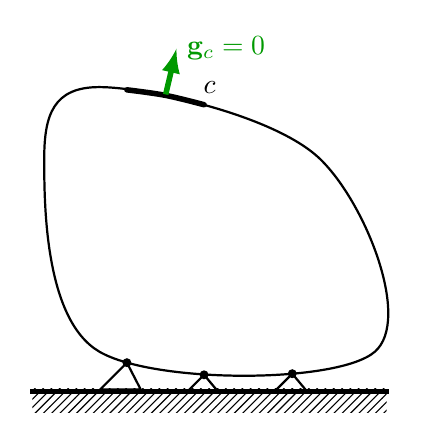
\begin{tikzpicture}[scale=0.7]
\tikzstyle{ground}=[fill,pattern=north east lines,draw=none,minimum height=0.3cm,inner sep=0pt,outer sep=0pt]


	\draw [line width=2pt,black,cap=round]  plot[smooth, tension=.6] coordinates { (2.9,4.98) (2.2,5.15)  (1.5,5.25) };  
	\node[outer sep=0pt,thick] at (3,5.3) [] {$c$};
	
	\draw [line width=2pt,black!40!green,solid,-latex] plot[] coordinates { (2.2,5.15)  (2.4,6.) }; 
	
	\node[outer sep=0pt,thick] at (3.3,6) [black!40!green] {{$\mathbf{g}_{c}=0$}};
	
	
	\node (ground) [ground,anchor=south,minimum width=4.5cm,rotate = 0] at (3,-0.6) {};
%	\node () [anchor=south] at (3,-1.4) {Grounded support};
	\draw [line width=2pt,black,solid,-] plot[] coordinates { (-0.25,-0.22)  (6.25,-0.22) }; 
	
	
	\draw [thick]  plot[smooth cycle, tension=.6] coordinates {(0,4) (1,0.5) (6,0.5) (5,4) (1,5.3) };
	
	
	\draw[black,fill=black] (4.5,0.1) circle (2pt);
	\begin{scope}[xshift=4.5cm,yshift=0.1cm]
		\draw [thick]  plot[] coordinates {(0,0) (0.25,-0.3) (-0.3, -0.3) (0,0) };
	\end{scope}
	

		\draw[black,fill=black] (2.9,0.08) circle (2pt);
	\begin{scope}[xshift=2.9cm,yshift=0.08cm]
		\draw [thick]  plot[] coordinates {(0,0) (0.25,-0.3) (-0.3, -0.3) (0,0) };
	\end{scope}
	
	\draw[black,fill=black] (1.5,0.3) circle (2pt);
	\begin{scope}[xshift=1.5cm,yshift=0.3cm]
		\draw [thick]  plot[] coordinates {(0,0) (0.25,-0.485) (-0.485, -0.485) (0,0) };
	\end{scope}
	

\end{tikzpicture}
\end{document}
